% Figure clh_lean_sharp: the extremal pair of the sharp cotangent cycle inequality for two (eta, m).
% Illustrates CLH-12 (Theorem thm:sharp-cot). Inputs: (eta/pi, m) = (0.05, 4) and (0.02, 7).
% Source of the figure, typeset in the paper's own fonts (T1, Latin Modern, 11pt) at the paper's text
% width (6.5in), so \includegraphics does not rescale it. It adds no assertion.
% Every coordinate is read from numerical values computed by floating-point code that follows the
% paper's formulas (the pictures' Lean helper); the SHA-256 of each output line it comes from:
%   D108_sharp 464126a6156f853043e63ac1d377f76ab78a68fc1ec7153267d325fe6d8a17a9
%   D109_sharp_m7 e25e3bb91f922cc94e533edeb7114e1f0d8551b6e671eea0edf6796cda09d267
% Build: pdflatex <this file> && pdftocairo -svg <this file>.pdf <this file>.svg

\documentclass[11pt]{standalone}
\usepackage[T1]{fontenc}
\usepackage{lmodern}
\usepackage{amsmath,amssymb}
\usepackage{tikz}
\usetikzlibrary{arrows.meta,calc}

% the palette of the paper's other figures: blue solid for the first object, ochre dashed for the second
\definecolor{ink}{HTML}{233740}
\definecolor{muted}{HTML}{65757D}
\definecolor{pblue}{HTML}{0072B2}
\definecolor{qochre}{HTML}{B87827}

\tikzset{
  ax/.style={draw=muted, line width=0.5pt},
  axd/.style={draw=muted!70, line width=0.4pt, dash pattern=on 1.5pt off 2pt},
  tick/.style={draw=muted, line width=0.5pt},
  lab/.style={font=\footnotesize, inner sep=1.2pt, text=ink},
  labm/.style={font=\small, inner sep=1.2pt, text=ink},
  labw/.style={font=\footnotesize, inner sep=1pt, text=ink, fill=white, fill opacity=0.8, text opacity=1},
  labP/.style={font=\footnotesize, inner sep=1.2pt, text=pblue},
  labQ/.style={font=\footnotesize, inner sep=1.2pt, text=qochre},
  tk/.style={font=\footnotesize, inner sep=1pt, text=muted},
  panel/.style={font=\small, inner sep=0pt, text=ink},
  curveP/.style={pblue, line width=1.1pt, line cap=round, line join=round},
  thinP/.style={pblue, line width=0.8pt, line cap=round, line join=round},
  thinQ/.style={qochre, line width=0.8pt, dash pattern=on 3pt off 1.6pt, line cap=round, line join=round},
  curveQ/.style={qochre, line width=1.1pt, dash pattern=on 4pt off 1.6pt, line cap=round},
  fillP/.style={pblue, fill=pblue!8, line width=1.1pt, line join=round},
  dotI/.style={circle, draw=ink, fill=ink, line width=0.6pt, inner sep=0pt, minimum size=4.6pt},
  dotIs/.style={circle, draw=ink, fill=ink, line width=0.5pt, inner sep=0pt, minimum size=3.2pt},
  ringI/.style={circle, draw=ink, fill=white, line width=0.6pt, inner sep=0pt, minimum size=4.6pt},
  dotP/.style={circle, draw=pblue, fill=pblue, line width=0.6pt, inner sep=0pt, minimum size=4.6pt},
  dotQ/.style={circle, draw=qochre, fill=qochre, line width=0.6pt, inner sep=0pt, minimum size=4.6pt},
  dotQs/.style={circle, draw=qochre, fill=qochre, line width=0.5pt, inner sep=0pt, minimum size=3pt},
  ringQ/.style={circle, draw=qochre, fill=white, line width=0.6pt, inner sep=0pt, minimum size=4.6pt},
}

\begin{document}
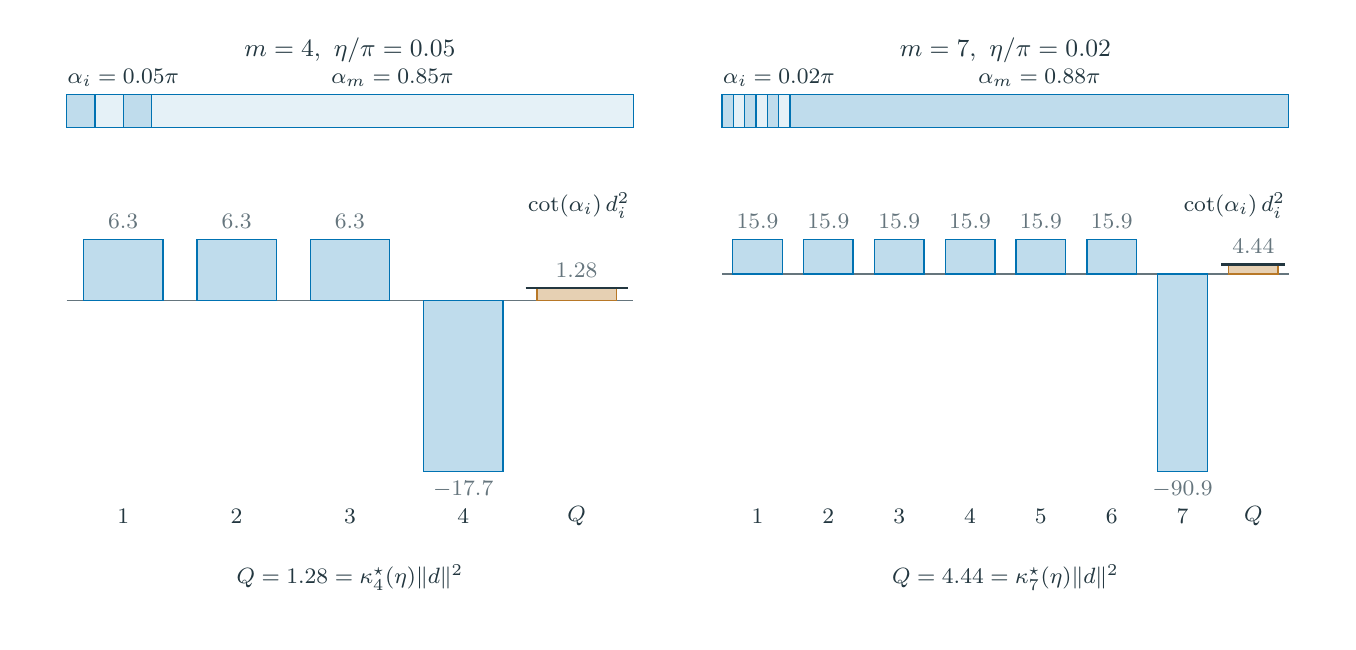
\begin{tikzpicture}[x=1bp,y=1bp]
\useasboundingbox (0bp,0bp) rectangle (468bp,214bp);
\node[labm] at (116.00,206.00) {$m=4,\ \eta/\pi=0.05$}; %t A-head
%box As 14 178 204 12 0 1 0 1
\draw[fill=pblue!25, draw=pblue, line width=0.5pt] (14.00,178.00) rectangle (24.20,190.00); %rect As/1 0 0.05
\draw[fill=pblue!10, draw=pblue, line width=0.5pt] (24.20,178.00) rectangle (34.40,190.00); %rect As/2 0.05 0.1
\draw[fill=pblue!25, draw=pblue, line width=0.5pt] (34.40,178.00) rectangle (44.60,190.00); %rect As/3 0.1 0.15
\draw[fill=pblue!10, draw=pblue, line width=0.5pt] (44.60,178.00) rectangle (218.00,190.00); %rect As/4 0.15 1
\node[lab, anchor=west] at (13.00,196.00) {$\alpha_i=0.05\pi$}; %num A-eta 0.05
\node[lab] at (131.30,196.00) {$\alpha_m=0.85\pi$}; %num A-last 0.85
%box At 14 46 204 100 0 5 -20.06121916 8.711476121
\draw[ax] (14.00,115.72) -- (218.00,115.72); %line
\draw[fill=pblue!25, draw=pblue, line width=0.5pt] (20.12,115.72) rectangle (48.68,137.67); %bar At/0 6.313751515
\node[tk] at (34.40,144.17) {$6.3$}; %num A-val0 6.3
\node[lab] at (34.40,38.00) {$1$}; %t A-idx0
\draw[fill=pblue!25, draw=pblue, line width=0.5pt] (60.92,115.72) rectangle (89.48,137.67); %bar At/1 6.313751515
\node[tk] at (75.20,144.17) {$6.3$}; %num A-val1 6.3
\node[lab] at (75.20,38.00) {$2$}; %t A-idx1
\draw[fill=pblue!25, draw=pblue, line width=0.5pt] (101.72,115.72) rectangle (130.28,137.67); %bar At/2 6.313751515
\node[tk] at (116.00,144.17) {$6.3$}; %num A-val2 6.3
\node[lab] at (116.00,38.00) {$3$}; %t A-idx2
\draw[fill=pblue!25, draw=pblue, line width=0.5pt] (142.52,115.72) rectangle (171.08,54.33); %bar At/3 -17.66349455
\node[tk] at (156.80,47.83) {${-}17.7$}; %num A-val3 -17.7
\node[lab] at (156.80,38.00) {$4$}; %t A-idx3
\draw[fill=qochre!35, draw=qochre, line width=0.5pt] (183.32,115.72) rectangle (211.88,120.16); %bar At/4 1.277759994
\node[tk] at (197.60,126.66) {$1.28$}; %num A-val4 1.28
\node[lab] at (197.60,38.00) {$Q$}; %t A-idx4
\draw[ink, line width=0.8pt] (179.24,120.16) -- (215.96,120.16); %kline At 1.277759994
\node[lab, anchor=east] at (218.00,150.00) {$\cot(\alpha_i)\,d_i^{2}$}; %t A-term
\node[lab] at (116.00,16.00) {$Q=1.28=\kappa_{4}^{\star}(\eta)\lVert d\rVert^{2}$}; %num A-eq 1.28
\node[labm] at (352.00,206.00) {$m=7,\ \eta/\pi=0.02$}; %t B-head
%box Bs 250 178 204 12 0 1 0 1
\draw[fill=pblue!25, draw=pblue, line width=0.5pt] (250.00,178.00) rectangle (254.08,190.00); %rect Bs/1 0 0.02
\draw[fill=pblue!10, draw=pblue, line width=0.5pt] (254.08,178.00) rectangle (258.16,190.00); %rect Bs/2 0.02 0.04
\draw[fill=pblue!25, draw=pblue, line width=0.5pt] (258.16,178.00) rectangle (262.24,190.00); %rect Bs/3 0.04 0.06
\draw[fill=pblue!10, draw=pblue, line width=0.5pt] (262.24,178.00) rectangle (266.32,190.00); %rect Bs/4 0.06 0.08
\draw[fill=pblue!25, draw=pblue, line width=0.5pt] (266.32,178.00) rectangle (270.40,190.00); %rect Bs/5 0.08 0.1
\draw[fill=pblue!10, draw=pblue, line width=0.5pt] (270.40,178.00) rectangle (274.48,190.00); %rect Bs/6 0.1 0.12
\draw[fill=pblue!25, draw=pblue, line width=0.5pt] (274.48,178.00) rectangle (454.00,190.00); %rect Bs/7 0.12 1
\node[lab, anchor=west] at (249.00,196.00) {$\alpha_i=0.02\pi$}; %num B-eta 0.02
\node[lab] at (364.24,196.00) {$\alpha_m=0.88\pi$}; %num B-last 0.88
%box Bt 250 46 204 100 0 8 -101.6076374 26.57656141
\draw[ax] (250.00,125.27) -- (454.00,125.27); %line
\draw[fill=pblue!25, draw=pblue, line width=0.5pt] (253.82,125.27) rectangle (271.68,137.67); %bar Bt/0 15.89454484
\node[tk] at (262.75,144.17) {$15.9$}; %num B-val0 15.9
\node[lab] at (262.75,38.00) {$1$}; %t B-idx0
\draw[fill=pblue!25, draw=pblue, line width=0.5pt] (279.32,125.27) rectangle (297.18,137.67); %bar Bt/1 15.89454484
\node[tk] at (288.25,144.17) {$15.9$}; %num B-val1 15.9
\node[lab] at (288.25,38.00) {$2$}; %t B-idx1
\draw[fill=pblue!25, draw=pblue, line width=0.5pt] (304.82,125.27) rectangle (322.68,137.67); %bar Bt/2 15.89454484
\node[tk] at (313.75,144.17) {$15.9$}; %num B-val2 15.9
\node[lab] at (313.75,38.00) {$3$}; %t B-idx2
\draw[fill=pblue!25, draw=pblue, line width=0.5pt] (330.32,125.27) rectangle (348.18,137.67); %bar Bt/3 15.89454484
\node[tk] at (339.25,144.17) {$15.9$}; %num B-val3 15.9
\node[lab] at (339.25,38.00) {$4$}; %t B-idx3
\draw[fill=pblue!25, draw=pblue, line width=0.5pt] (355.82,125.27) rectangle (373.68,137.67); %bar Bt/4 15.89454484
\node[tk] at (364.75,144.17) {$15.9$}; %num B-val4 15.9
\node[lab] at (364.75,38.00) {$5$}; %t B-idx4
\draw[fill=pblue!25, draw=pblue, line width=0.5pt] (381.33,125.27) rectangle (399.17,137.67); %bar Bt/5 15.89454484
\node[tk] at (390.25,144.17) {$15.9$}; %num B-val5 15.9
\node[lab] at (390.25,38.00) {$6$}; %t B-idx5
\draw[fill=pblue!25, draw=pblue, line width=0.5pt] (406.83,125.27) rectangle (424.67,54.33); %bar Bt/6 -90.92562082
\node[tk] at (415.75,47.83) {${-}90.9$}; %num B-val6 -90.9
\node[lab] at (415.75,38.00) {$7$}; %t B-idx6
\draw[fill=qochre!35, draw=qochre, line width=0.5pt] (432.33,125.27) rectangle (450.17,128.73); %bar Bt/7 4.441648243
\node[tk] at (441.25,135.23) {$4.44$}; %num B-val7 4.44
\node[lab] at (441.25,38.00) {$Q$}; %t B-idx7
\draw[ink, line width=0.8pt] (429.77,128.73) -- (452.73,128.73); %kline Bt 4.441648243
\node[lab, anchor=east] at (454.00,150.00) {$\cot(\alpha_i)\,d_i^{2}$}; %t B-term
\node[lab] at (352.00,16.00) {$Q=4.44=\kappa_{7}^{\star}(\eta)\lVert d\rVert^{2}$}; %num B-eq 4.44
\end{tikzpicture}
\end{document}
